\documentclass[10pt,twocolumn,a4paper]{pizzato}

\usepackage[utf8]{inputenc}
\usepackage[T1]{fontenc}
\usepackage[brazil]{babel}

%\usepackage{lmodern}
\usepackage{times}

\begin{document}

\title{Título do experimento}
\author{?. ?. ?????}
\turma{??}
\cartao{?????}
\email{?????@ufrgs.br}

\resumo{O resumo deve conter de forma fiel, breve e concisa os aspectos mais relevantes do trabalho realizado, na mesma progressão com que os assuntos são discutidos ao longo do texto. É indispensável que apresente um panorama geral do trabalho de forma clara e objetiva. A redação deve ser elaborada em parágrafo único, com sujeito indeterminado expresso pela 3ª pessoa do singular e de sorte que qualquer leitor seja capaz de compreendê-la. Sua extensão é de no máximo 100 palavras}
\keywords{????. ????. ????.}

\maketitle


\section*{Preparação do relatório}
Os autores deverão preparar seus relatórios utilizando a estrutura apresentada neste documento. Este é o modelo de relatório a ser adotado na disciplina, o qual pode ser copiado do endereço \url{http://chasqueweb.ufrgs.br/~roger.pizzato/201102/ENG04404/mr.doc}. O arquivo contido no endereço anterior já encontra-se formatado para a elaboração do relatório, ao estilo de um artigo científico usualmente observado na literatura. Para a redação deste último, utilize algum editor de texto com código livre baseado no núcleo \textit{StarOffice} disponibilizado pela \textit{Sun Microsystems}. Recomendo fortemente que os autores utilizem o pacote \textit{BrOffice}, com cópia livre no endereço \url{http://www.broffice.org}. Os autores devem dominar as funções principais desta ferramenta de edição de texto. Será importante para as demais disciplinas no decorrer de seus Cursos.

O relatório será entregue \textbf{sempre} no início da aula consecutivamente posterior à realização da atividade experimental, em mãos, ao professor. Relatórios entregues fora do prazo acima estabelecido não serão avaliados, sendo portanto a estes atribuído grau \textbf{zero}. Relatórios plagiados, em inteiro ou parcial teor, não serão igualmente avaliados. Estes também receberão grau \textbf{zero} e serão submetidos ao órgão competente da UFRGS para a devida sanção disciplinar. Leia na íntegra o Regimento Geral da Universidade no endereço \url{http://www.ufrgs.br/consun/regimento\_geral.pdf} para a descrição das sanções disciplinares cabíveis neste caso.

As figuras podem ser inseridas em uma coluna, conforme apresenta a figura \ref{Fig1}, ou sobre duas colunas, conforme demonstra a figura \ref{Fig2}. Prepare seu gráfico ou figura em seu programa de preferência e a exporte em algum formato que utilize compactação (JPEG, GIF, PNG, TIFF dentre outros). Tais arquivos são menores que os demais e reduzem o tamanho do arquivo final que contém o relatório completo. O autor pode, ainda, se assim preferir, inserir a figura como objeto.

Se houver qualquer dúvida com relação a formatação de qualquer parte integrante do relatório, consulte as normas da Associação Brasileira de Normas Técnicas (ABNT) no endereço \url{http://www.abnt.org.br/}. É esta a Instituição legalmente habilitada no País para a normatização de qualquer trabalho técnico e/ou científico.

Tais como as figuras, as Tabelas também podem ser inseridas em uma ou duas colunas. Vide respectivamente as Tabelas \ref{Tab1} e \ref{Tab2} para exemplificação.

\begin{figure}[h]
    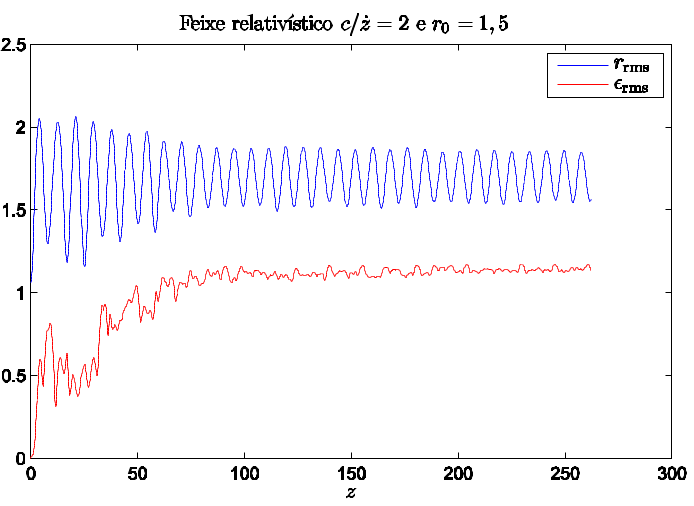
\includegraphics[width=\columnwidth]{Fig1.png}
    \caption{Exemplo de figura inserida em uma coluna}    
    \label{Fig1}
\end{figure}


Tanto as figuras quanto as tabelas devem estar centralizadas na(s) coluna(s) e nestas deve ser inserida uma legenda. Nas figuras, as legendas posicionam-se na parte inferior enquanto, nas Tabelas, estas posicionam-se na parte superior. As legendas devem estar justificadas na(s) coluna(s) e serem breves e concisas. Devem ser antecedidas de palavra designativa, seguida do número arábico que represente sua ordem de ocorrência no relatório, do caractere “:” e finalmente do seu respectivo texto explicativo. Não deve ser acrescentado ponto ao término do texto explicativo. Observe as Figuras \ref{Fig1} e \ref{Fig2} e as Tabelas \ref{Tab1} e \ref{Tab2} para exemplificação.

\begin{table}[h]
    \centering
    \caption{Exemplo de tabela inserida em uma coluna}
    \label{Tab1}
    \begin{tabular}{ c c c }
    \hline
    \hline
    $z$ & $r_{\text{rms}}$ & $\varepsilon_{\text{rms}}$ \\ \hline
    0   & 0,85 & 0    \\
    50  & 1,65 & 0,82 \\
    100 & 1,51 & 1,22 \\
    \hline
    \hline
    \end{tabular}
\end{table}

\begin{figure*}[t]
    \centering
    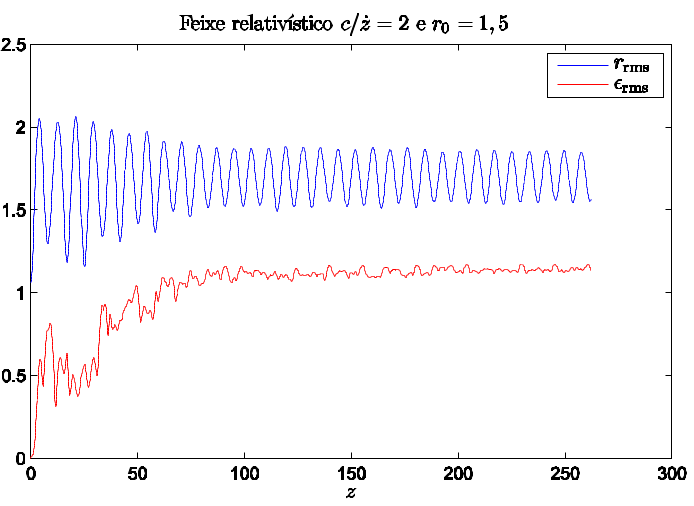
\includegraphics[width=0.8\textwidth]{Fig2.png}
    \caption{Exemplo de figura inserida em 2 colunas}    
    \label{Fig2}
\end{figure*}

\begin{table*}[t]
    \centering
    \caption{Exemplo de tabela inserida em duas colunas}
    \label{Tab2}
    \begin{tabular}{ c c c l }
    \hline
    \hline
    $z$ & $r_{\text{rms}}$ & $\varepsilon_{\text{rms}}$ & Descrição \\ \hline
    0   & 0,85 & 0    & Feixe inicialmente frio\\
    50  & 1,65 & 0,82 & Feixe morno, esquentando\\
    100 & 1,51 & 1,22 & Feixe quente, termalizado\\
    \hline
    \hline
    \end{tabular}
\end{table*}

As Figuras e as Tabelas devem ser citadas ao longo do trabalho com o mesma palavra designativa utilizada em sua legenda. Toda a figura e tabela deve associadamente possuir um parágrafo explicativo ao longo do relatório. Figuras e Tabelas que não forem citadas e assim descritas ao longo do relatório devem ser obrigatoriamente excluídas.

As equações importantes do relatório devem ser inseridas mediante uma tabela de 1 linha e 2 colunas, sem qualquer borda gráfica. Na primeira coluna, a maior, insere-se centralizadamente a equação e na segunda, a menor, alinhado à direita, insere-se o número arábico que determina a sua ordem de ocorrência no relatório. As equações secundárias, com menor relevância no contexto do relatório, podem ser inseridas no corpo do texto e não requerem numeração específica. Para exemplificação, considere sendo $j = \sqrt{-1}$

\begin{equation}
    e^{j \theta} = \text{cos($\theta$)} + j \text{cos($\theta$)}
\end{equation}

O relatório deve possuir – no máximo – 2 páginas. Embora o corpo do relatório deva ser redigido em preto, as figuras, se assim necessário, podem utilizar quaisquer cores. Prefira aquelas cores que produzam contraste suficiente para uma leitura confortável. A impressão obrigatoriamente deve acompanhar as cores com as quais o trabalho foi elaborado. Se houver figuras coloridas, a impressão deve ser obrigatoriamente colorida. Caso haja impossibilidade de impressão com cores, então necessariamente elabore as figuras apenas com preto e branco (ou obviamente na escala de cinzas). Caso a impressão ocorra em computador diverso daquele na qual o relatório foi redigido, prefira formatos de arquivos que ofereçam perfeita portabilidade, tais como o .pdf, incluindo as fontes utilizadas. O autor deve condicionar a elaboração do seu relatório considerando os recursos computacionais que dispõe. O tamanho do papel utilizado deve ser A4 (210 mm de largura por 297 mm de altura).

Por precaução, o autor deve acostumar-se a salvar periodicamente o seu relatório. Programe o seu Editor para que automatize esta tarefa. Na eventualidade de qualquer interrupção imprevista, o retrabalho é minimizado.

O autor deve revisar minuciosamente o seu relatório. O texto que o autor elabora é aquilo que representa o seu trabalho. É irrelevante desenvolver um bom trabalho se a sua efetiva documentação é precária e deficiente. É desagradável a leitura de relatórios com erros graves de grafia e concordância. Assim, após leitura minuciosa, utilize do corretor ortográfico para que eventuais erros sejam minimizados. Mais: o relatório será avaliado apenas em relação a aquilo que contém registrado. Desta forma, os autores são encorajados a descrever todas as atividades desenvolvidas, obviamente sempre observando objetividade e síntese, qualidades estas imprescindíveis em uma redação técnico-científica. Na eventualidade da não-existência de um termo em português para certo jargão técnico em inglês, abdique da língua vernácula e utilize a estrangeira, destacada por \textit{itálico}.

Referências bibliográficas devem ser obrigatoriamente citadas ao longo do relatório \cite{furaste}. Caso alguma bibliografia tenha sido utilizada mas não efetivamente citada ao longo do relatório, prefira a adoção do termo obras consultadas.

A redação de um relatório deve atender a uma ampla audiência. Portanto, reforça-se aos autores: o texto deve ser claro o suficiente de sorte que alguém que não realizou a atividade experimental possa, a partir do relatório elaborado, reproduzir não apenas o experimento, mas como também obter resultados semelhantes.

\section*{A estrutura do Relatório}

A estrutura do relatório prevista consta detalhadamente descrita a seguir.

\subsection*{Resumo}
Como já foi abordado acima, o resumo do relatório deve conter uma descrição sucinta e concisa do trabalho desenvolvido e dos resultados obtidos. Para motivar a sua leitura, é importante o autor destacar as informações relevantes aferidas com o trabalho.

\subsection*{Introdução}
A introdução deve contextualizar o assunto objeto do trabalho ao leitor. Em artigos científicos, é praxe a introdução recapitular os trabalhos já desenvolvidos no tema e documentados na literatura. Citações de muitas bibliografias assim são esperadas. Deve conter explicitamente o fenômeno físico a ser investigado e os objetivos associados com a realização do experimento. É imprescindível também que a teoria sob a qual o experimento baseia-se seja descrita.

\subsection*{Procedimento Experimental}
Nesta seção são descritos os procedimentos experimentais adotados, equipamentos adotados, os métodos de medida e os cálculos associados. Deve-se descrever em detalhe todos os aspectos anteriormente mencionados, de sorte que a reprodutibilidade dos resultados seja possível. Utilize de diagramas esquemáticos para que a compreensão seja facilitada. Importante: não trata-se de uma cópia do roteiro do experimento, uma vez que este último não contém os detalhes relevantes que somente podem ser percebidos durante a elaboração do experimento.

\subsection*{Resultados e Discussão}
É uma das partes mais importantes, pois traduz a qualidade do experimento desenvolvido. Nesta seção, os resultados aferidos com o experimento são apresentados na forma de tabelas, gráficos e diagramas. Os resultados experimentais devem ser confrontados com as previsões teóricas e com os resultados existentes na literatura citada na introdução.

No caso de os resultados experimentais, dentro da incerteza estimada, apresentarem discrepâncias com as previsões teóricas, o procedimento experimental deverá ser cuidadosamente revisto.

Recorde que todas as medidas realizadas possuem certa incerteza associada. Represente portanto o resultado da forma descrita nas aulas introdutórias, contendo o intervalo de variabilidade. No caso de uma medida de uma grandeza $x$ , represente-a portanto por $(\bar{x}+\Delta x)$, sendo $\bar{x}$ a média e $\Delta x$ o desvio padrão da média das medidas obtidas \cite{vuolo}. Adote sempre unidades do SI e considere a incerteza calculada com no máximo 2 dígitos significativos, conforme estabelece a ABNT.


\subsection*{Conclusão}
A conclusão deve abordar brevemente o experimento efetuado, os resultados obtidos e a sua compatibilidade com os objetivos estabelecidos na introdução. Se possível, o autor deve discutir a repercussão dos resultados e delinear os eventuais futuros trabalhos decorrentes.

\subsection*{Referências bibliográficas}
Nesta seção, apenas as bibliografias referenciadas durante a elaboração do relatório devem ser especificadas. As referências bibliográficas são indexadas por um número arábico que está vinculado com a sua ordem cronológica de citação ao longo do relatório. Considere o formato de redação abaixo especificado para as referências bibliográficas.

\begin{thebibliography}{9}

\bibitem{furaste} 
\textbf{P. A. Furasté.} \textit{Normas Técnicas para o trabalho científico – elaboração e formatação.} 14ª edição ampliada e reformulada. Porto Alegre: s.n., 2006.
 
\bibitem{vuolo} 
\textbf{J. H. Vuolo.} \textit{Fundamentos da Teoria de Erros.} 2ª edição. Rio de Janeiro: Editora Edgard Blücher LTDA, 1996.
\end{thebibliography}

\end{document}